\chapter{Actors and Their Supervision}
\label{supervision_model}

\section{Actor Programming}

An actor responses to messages it receives ...


The Actor model defined by \citet{Hewitt:1973} treats actors as
primitive computational components.  Actors collaborate by sending asynchronous
messages to each other.  An actor independently determines its reaction to
messages it receives.

blah blah

\section{The Supervision Tree}
A supervision tree, first proposed in the Erlang OTP library 
\citep{OTP}, consists of two types of actors: workers and supervisors. A worker 
implements part of the business logic and reacts to request messages.  A 
supervisor is responsible for initializing and monitoring its children, which 
are workers or supervisors for other actors, and restarting its children when 
necessary.  The behaviour of a supervisor is defined by its {\it supervisor 
strategies}.

To study the properties of the supervision tree and compare design 
alternatives, an extensible formal model is required to capture the essence of 
the supervision tree. In this thesis, worker and supervisor are modelled as 
different Deterministic Finite Automata (DFAs) (Section 
\ref{supevision_node_model}).  A supervision tree (Section 
\ref{supevision_tree_model}) has supervisors as its internal nodes and workers 
as its leaf nodes.  Further analyses (Section \ref{supervision_unifying}) show 
that attempts of unifying a supervisor node and a worker node result in 
problems or complexity.  Our model analysis concludes with implementation 
suggestions given in Section \ref{supervision_implementaion}.

\subsection{Worker and Supervisor as Deterministic Finite Automata (DFAs)} 
\label{supevision_node_model}

\begin{figure}[p]
%     \centering 
\begin{adjustwidth}{-2.5cm}{} 
        \subfigure[Worker]{
            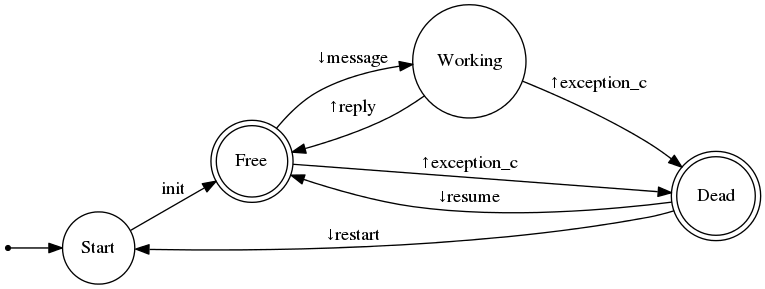
\includegraphics[scale=0.7]{child.png}
%            \caption{A gull}
            \label{fig:sup_node_1}
        }\\
        \subfigure[Supervisor]{
           \label{fig:sup_node_2}
           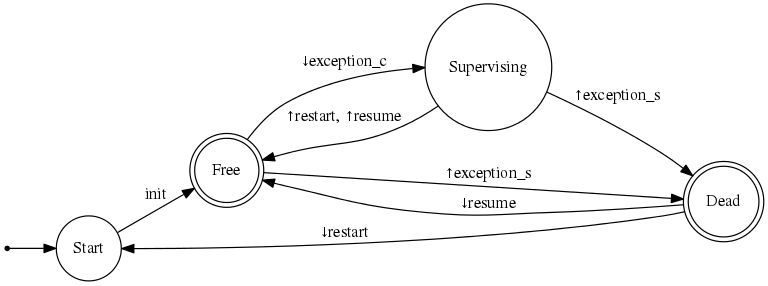
\includegraphics[scale=0.7]{supervisor.png}
        }\\
  \caption{Worker and Supervisor as Deterministic Finite Automata}
 \end{adjustwidth}      
  \label{fig:DFA}        
\end{figure}



Figure \ref{fig:DFA} gives the state graphs of DFAs that describe 
worker and supervisor in a supervision tree.  Nodes in the graphs represent 
states of that DFA and arrows are transitions from one state to another.  A 
transition is triggered either by the node itself or due to changes of the 
environment it resides.

At any time, a worker may be in one of its four states: {\bf Start}, {\bf 
Free}, {\bf Working}, or {\bf Dead}.  After automatically being initialized to 
the {\bf Free} state, the worker can receive a messages from its outside 
environment and enters into the {\bf Working} state where no other messages 
will be processed.  If no error occurred when processing the message, the 
worker returns a result and go back to the {\bf Free} state.  An error may 
occur during the middle of message processing (e.g. software bugs) or when the 
environment changes (e.g. hardware failures), in which cases the worker reports 
its failure to its supervisor and goes to the {\bf Dead} state.  A dead worker 
can be resumed (with the restored internal state) or restarted (with an initial 
internal state) by its supervisor so that it can process new messages.  The 
{\bf Free} and {\bf Dead} states are marked as accept states from which no 
further actions may occur.  On the contrary, a {\bf Working} worker will 
eventually emit a reply message or raise an exception; and all workers will be 
successfully initialized.

Similarly, Figure \ref{fig:sup_node_2} gives the DFA of a supervisor whose only 
duty is supervising its children.  A supervisor that in its {\bf Free} state 
reacts to failure messages from its children.  Meanwhile, a supervisor may fail 
at any time and reports its failure to its supervisor.

\subsection{The Supervision Relationship and Supervisor Strategies}
\label{supevision_tree_model}

\begin{figure}[h]
 \label{supevision_tree_fig} 
 \begin{tabular}{r c l l l}
 SupTree & =   & Worker &&\\
         & $|$ & OneForOne$_D$  & Sup & [SupTree] \\
         & $|$ & OneForAll$_D$  & Sup & [SupTree] \\
         & $|$ & RestForOne$_D$ & Sup & [SupTree] \\
         & $|$ & $\cdots$ &&\\
\\
 D & = & \multicolumn{3}{c}{Escalate $|$ Restart $|$ Resume $|$ 
Stop $|$ $\cdots$ } \\
         
 \end{tabular}
 \caption{Supervision Tree}
\end{figure}

The structure of a supervision tree is straightforwardly defined in Figure 
\ref{supevision_tree_fig}.  Each internal node is labelled by a supervisor 
strategy which contains a behaviour function whose type is {\tt Exception 
$\Rightarrow$ Directive}, where {\tt Exception} is the type of failures raised 
by children and {\tt Directive} represents the final {\tt system action} for 
that failure.  Subtrees of a node is organized as a List.

There are 3 general supervisor strategies found in existing libraries: {\tt 
OneForOne}, {\tt AllForOne}, and {\tt RestForOne}.  If a supervisor adopts the
{\tt OneForOne} strategy, the behaviour function is applied to the failed child 
only. If a supervisor adopts the {\tt AllForOne} supervisor strategy, the 
behaviour function is applied to all children when any of them fails.  If a 
supervisor adopts the {\tt RestForOne} supervisor strategy, the behaviour 
function is applied to the failed child and children in the rest of the list.  
New supervisor strategies can be added to the model when required.

The Erlang OTP library \citep{OTP} implements all three supervisor strategies 
whereas the Akka library \citep{akka_api, akka_doc} does not implement the {\tt 
RestForOne} strategy because children in Akka is not ordered.  Simulating the 
{\tt RestForOne} supervisor strategy in Akka requires ad-hoc implementation 
that groups related children and defines special messages to trigger actor 
termination.  No evidence shows that the lack of the {\tt RestForOne} 
strategy will result in difficulties when rewriting Erlang applications in Akka.

There are 4 directives found in existing libraries: {\tt Escalate}, {\tt 
Restart}, {\tt Resume}, and {\tt Stop}.  The {\tt Escalate} directive throws 
the exception to the supervisor of the supervisor; the {\tt Restart} directive 
restart the failed child with its initial internal state; the {\tt Resume} 
directive restart the failed child with the restored internal state and ask the 
child to process the message again; finally, the {\tt Stop} directive
terminates the failed actor permanently.  New directives can be added to the 
model when required.

The Akka library \citep{akka_api, akka_doc} implements all four directives 
whereas the Erlang OTP library \citep{OTP} only provides the {\tt Restart} 
directive and the {\tt Stop} directive.  The {\tt Escalate} directive can be 
simulated in Erlang by manually defining a function that terminates the 
supervisor when one of its children fails.  The {\tt Resume} directive is not 
needed in Erlang OTP because an Erlang actor does not have a mutable internal 
state.


\subsection{Unifying Supervisor and Worker}
\label{supervision_unifying}

\begin{figure}[p]
%  \ContinuedFloat 
\begin{adjustwidth}{-2.5cm}{} 
        \subfigure[Supervisor AND Worker]{
            \label{fig:sup_node_3}
            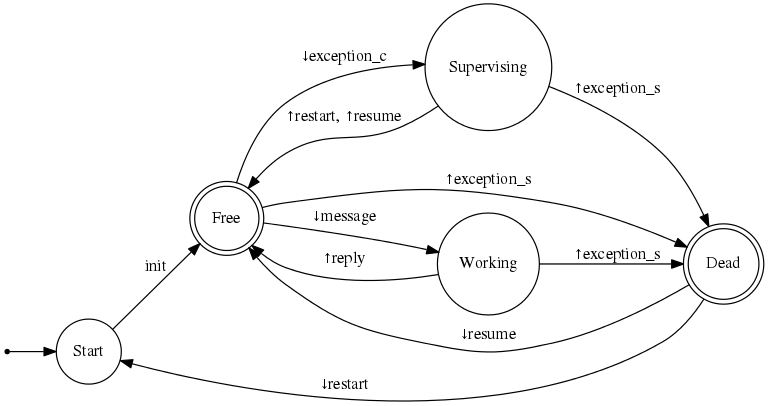
\includegraphics[scale=0.7]{supervisorANDchild.png}
        }\\
        \subfigure[Supervisor PAR Worker]{
            \label{fig:sup_node_4}
            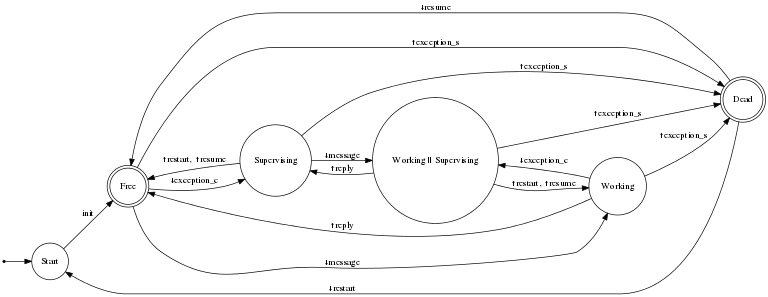
\includegraphics[scale=0.7]{supervisorPARchild.png}
        }\\
    \caption{A Node that Unifies Supervisor and Worker}
 \end{adjustwidth}    
   \label{fig:unify}
\end{figure}

Notice that the model for supervisor and worker are similar.  Can we define 
a {\it unified} model that matches both supervisor and worker?  Of course we 
can, and indeed there are three ways to do so.  This section will present three 
unified models and discuss the trade-off of using those models.

\paragraph{A General Actor Model}
The model for worker in Figure \ref{fig:sup_node_1} is no more than an actor 
that can be resumed or restarted when it fails.  If an exception raised from a 
child is viewed as a request message to its supervisor and a restart/resume 
command is viewed as a reply message to the child, the supervisor model (Figure 
\ref{fig:sup_node_2}) coincides with the worker model (Figure 
\ref{fig:sup_node_1}).  For this reason, in Erlang and Akka, both supervisors 
and workers are implemented as actors.  Defining supervisors and workers in 
terms of the general actor model is a reasonable implementation strategy; 
however, a specialized model for supervisor is desired in model analyses so 
that properties and behaviours of supervisors can be better discussed.

\paragraph{Combining Supervisor and Worker}  

The supervision tree defined in Section \ref{supevision_tree_model} requires 
supervisors as its internal nodes and workers as its leaves.  In contrast, the 
Akka library adopts the alternative design where an internal node can be both a 
supervisor for other nodes and a worker that implements part of the business 
logic.  The supervisor process and the worker process in Akka share the message 
box and are compounded to the message handler of the actor.  Figure 
\ref{fig:sup_node_3} gives a DFA that models the internal node of an Akka 
supervision tree.  It is clear that the internal node cannot restart or resume 
failed child when it is processing a message for other purposes, and it cannot 
perform a computational task when it carries out its duty as a supervisor.  In 
both cases, the performance of the system suffers.

\paragraph{Supervisor in Parallel with Worker}  One way to get around the 
limitation of the above design is executing the supervision process and the 
worker process in parallel, as shown in Figure \ref{fig:sup_node_4}.  
From the perspective of model analysis, the above parallel model is equivalent 
to the one which separates the supervisor process and the worker process into 
two nodes, and treat them either as siblings or as a supervisor and a child.  
Of course additional dependencies of the life cycle of those two logically 
separated nodes shall be addressed in the sense that the failure of one node 
will cause the failure of the other.

\vspace{15 pt}

To summarize, a node that naively combining the role of supervisor and worker 
(Figure \ref{fig:sup_node_3}) has less availability than a node that place the 
supervision process and the worker process in parallel (Figure 
\ref{fig:sup_node_4}).  Interestingly, during the process of designing and 
implementing the TAkka library (Chapter \ref{takka_design}), we realized that 
the type of supervision messages should be separated 
from the type of other messages.  However, partly because we would like to 
reuse the Akka implementation and partly because we did not have the above 
model at that time, the process of handling supervision messages is not 
separated from the process of handling other messages.


\subsection{Implementation Considerations}
\label{supervision_implementaion}

The two DFAs given in Figure \ref{fig:DFA} are abstracted for model analyses.  
In an implementation of the supervision tree model, following issues might be 
considered.

\paragraph{Distributed Deployment}
Supervision Tree represents the logic relationship between nodes.  In 
practice, nodes of a supervision tree may be deployed in distributed machines.  
A child node may be restarted at or shipped to another physical or virtual 
machine but stays in the same local position of the supervision tree.


\paragraph{Heart-Beat Message}  At run-time, failures may occur at any time 
for different reasons.  In some circumstances, failure messages of a child may 
not be delivered to its supervisor, or even worse, not be sent by the failed 
child at all.  To build a system tolerant to the above failures, supervisors 
need to be aware of the liveness of their children.  One commonly used approach 
is asking the child to periodically send heart-beat messages to 
its supervisor.  If no heart-beat message is received from a child within a 
time-out, that child is considered dead by the supervisor and an appropriate 
recovery process is activated.  In our model, a logical exception is sent from a 
child to its supervisor when no heart-beat message is delivered within a 
time-out, and a restart or resume message is sent to a suitable (virtual) 
machine where the recovered node will reside.

\paragraph{Message Queuing}
In the model given in Figure \ref{fig:sup_node_1}, a node can processed one 
message a time when it is {\bf Free}.  The model does not exclude the case 
where messages are queuing either in memory or a distributed database.  
Similarly, when a node is resumed from a failure, the message it was processing 
before that failure may either be restored or be discarded.


\section{Akka Basics}

\subsection{Akka Actor}
\label{akka actor}


An Akka Actor has four essential components as shown in Figure 
\ref{fig:akka_actor_api}: (i) a receive function that defines its reaction to 
incoming messages, (ii) an actor reference pointing to  itself, (iii) the actor 
 context representing the outside world of the actor, and (iv) the supervisor 
strategy for its children.

\begin{figure}[h]
\label{fig:akka_actor_api}
\begin{lstlisting}[language=scala]
package akka.actor
trait Actor{
  def receive:Any=>Unit
  val self:ActorRef
  val context:ActorContext
  var supervisorStrategy: SupervisorStrategy
}
\end{lstlisting}
\caption{Akka Actor API}
\end{figure}

Figure \ref{akkastring} shows an example actor in Akka.  The {\tt receive} 
function of the Akka actor has type {\tt Any$\Rightarrow$Unit} but the 
defined actor, {\tt ServerActor}, is only intended to process strings.  At Line 
16, a {\tt Props}, an abstraction of actor creation, is initialized and passed 
to an actor system, which creates an actor with name \textcolor{mauve}{\tt 
server} and returns a reference pointing to that actor.  Another way to obtain 
an actor is using the {\tt actorFor} method as shown in line 24.  We then use 
actor references to send the actor string messages and integer messages.  
String messages are processed in the way defined by the receive function.

\begin{figure}[p]
 \label{akkastring}
      \begin{lstlisting}[language=scala]
class ServerActor extends Actor {
  def receive = {
    case m:String => println("received message: "+m)
  }
}

class MessageHandler(system: ActorSystem) extends Actor {
  def receive = {
    case akka.actor.UnhandledMessage(message, sender, recipient) =>
      println("unhandled message:"+message);
  }
}

object ServerTest extends App {
  val system = ActorSystem("ServerTest")
  val server = system.actorOf(Props[ServerActor], "server")
  
  val handler = system.actorOf(Props(new MessageHandler(system)))
  system.eventStream.subscribe(handler,
                     classOf[akka.actor.UnhandledMessage]);
  server ! "Hello World"
  server ! 3
  
  val serverRef = system.actorFor("akka://ServerTest/user/server")
  serverRef ! "Hello World"
  serverRef ! 3
}


/*
Terminal output:
received message: Hello World
unhandled message:3
received message: Hello World
unhandled message:3
*/
    \end{lstlisting}
    \caption{A String Processor in Akka}
\end{figure}

Undefined messages are treated differently in different actor libraries.  In
Erlang, an actor keeps undefined messages in its mailbox, attempts to process
the message again when a new message handler is in use.  In versions prior to
2.0, an Akka actor raises an exception when it processes an undefined message.
In recent Akka versions, an undefined message is discarded by the actor and an
{\tt UnhandledMessage} event is pushed to the event stream of the actor system.
The event stream may be subscribed by other actors who are interested in
particular event messages.  To handle the unexpected integer message in the
above short example, an event handler is defined and created with 6 lines of 
code.


\subsection{Supervision}
\label{akkasup}

The Supervision Tree principle is proposed but optional in Erlang.  On the contrary,
the Akka library makes supervision obligatory by restricting the way of 
creating actors. Actors can only be initialized by using the {\tt actorOf}
method provided by {\tt ActorSystem} or {\tt ActorContext}.  Each actor system
provides a guardian actor for all user-created actors.  Calling the {\tt
actorOf} method of an actor system creates an actor supervised by the 
guardian actor.  Calling the {\tt actorOf} method of an actor context 
creates a child actor supervised by that actor.  Therefore, all user-created  
actors in an actor system, together with the guardian actor of that actor 
system, form a tree structure.  Obligatory supervision unifies the 
structure of actor deployment and simplifies the work of system maintenance.

Each actor in Akka is associated with an actor path.  The string representation
of the actor path of a guardian actor has format 
{\it akka://mysystem@IP:port/user}, where {\it mysystem} is the name of the 
actor system, {\it IP} and {\it port} are the IP address and the 
port number which the actor system listens to, and {\it user} is the name of 
the guardian actor.  The actor path of a child actor is actor path of its 
supervisor appended by the name of the child actor, either a user specified 
name or a system generated name.

Figure \ref{supervisedcalculator} defines a simple calculator which supports
multiplication and division. The simple calculator does not consider the
problematic case of dividing a number by 0, where an {\tt
ArithmeticException} will be raised.  We then define a safe calculator as the 
supervisor of the simple calculator.  The safe calculator delegates 
calculation tasks to the simple calculator and restarts the simple calculator 
when an {\tt ArithmeticException} is raised.  The supervisor strategy of
the safe calculator also specifies the maximum number of failures its child may 
have within a given time range.  If the child fails more frequently than the 
allowed frequency, the safe calculator will be  stopped, and its failure will be
reported to its supervisor, the system guardian actor in this example.  The
terminal output shows that the simple calculator is restarted before the third 
message and the fifth message are delivered.  The last message is not processed
because both calculators are terminated since the simple calculator fails more 
frequently than allowed.

\begin{figure}[p]
\label{supervisedcalculator}

  \begin{lstlisting}[language=scala]
case class Multiplication(m:Int, n:Int)
case class Division(m:Int, n:Int)

class Calculator extends Actor {
  def receive = {
    case Multiplication(m:Int, n:Int) =>
      println(m +" * "+ n +" = "+ (m*n))
    case Division(m:Int, n:Int) =>
      println(m +" / "+ n +" = "+ (m/n))
  }
}
class SafeCalculator extends Actor {
  override val supervisorStrategy =
    OneForOneStrategy(maxNrOfRetries = 2, withinTimeRange = 1 minute) {
      case _: ArithmeticException  =>
        println("ArithmeticException Raised to: "+self)
        Restart
    }
  val child:ActorRef = context.actorOf(Props[Calculator], "child")
  def receive = {    case m => child ! m  }
}
  val system = ActorSystem("MySystem")
  val actorRef:ActorRef = system.actorOf(Props[SafeCalculator],
"safecalculator")

  calculator ! Multiplication(3, 1)
  calculator ! Division(10, 0)
  calculator ! Division(10, 5)
  calculator ! Division(10, 0)
  calculator ! Multiplication(3, 2)
  calculator ! Division(10, 0)
  calculator ! Multiplication(3, 3)
/* Terminal Output:
3 * 1 = 3
java.lang.ArithmeticException: / by zero
ArithmeticException Raised to: Actor[akka://MySystem/user/safecalculator]
10 / 5 = 2
java.lang.ArithmeticException: / by zero
ArithmeticException Raised to: Actor[akka://MySystem/user/safecalculator]
java.lang.ArithmeticException: / by zero
3 * 2 = 6
ArithmeticException Raised to: Actor[akka://MySystem/user/safecalculator]
java.lang.ArithmeticException: / by zero
*/
    \end{lstlisting}
  \caption{Supervised Calculator}
\end{figure}




\begin{comment}
\section{Mixing Static and Dynamic Type Checking}
\label{type_checking}
A key advantages of static typing is that it detects some type errors at an 
early stage, i.e. at compile time.  The TAkka library is designed to detect 
type errors as early as possible.  Nevertheless, not all type errors can be 
statically detected, and some dynamic type checks are required. To address this 
issue, a notion of run-time type descriptor is required.

This section summarizes the type reflection mechanism in Scala and  explains
how it benefits the implementation of our typed name
server.  Our typed name server can be straightforwardly ported
to other platforms that support type reflection.

\subsection{Scala Type Descriptors}
Scala 2.8 defines a {\tt Manifest} class \footnote{Scala 2.10 introduces 
the Type class and the TypeTag class to replace Manifest.  At the time of this 
writing, TypeTag is not serializable as it should be due to bug SI-5919. } 
whose 
instance is a first class type descriptor used at runtime.  With the help of 
the {\tt Manifest} class, users can record the type information, including 
generic types, which may be erased by the JAVA compiler.  

In the Scala interactive session below, we obtain a Manifest value at Line 5 
and 
test a subtype relationship at Line 8.  To define a method that obtains type 
information of a generic type, Scala requires a type tag as an implicit 
argument to the method.  To simplify the API, Scala further provides a form of
syntactic sugar called context bounds.  We define a method using context
bounds at Line 11, which is compiled to the version using implicit 
arguments as shown at Line 12.


\begin{lstlisting}
scala> class Sup; class Sub extends Sup
defined class Sup
defined class Sub

scala> manifest[Sub]
res0: Manifest[Sub] = Sub

scala> manifest[Sub] <:< manifest[Sup]
res1: Boolean = true

scala> def getType[T:Manifest] = {manifest[T]}
getType: [T](implicit evidence$1: Manifest[T])Manifest[T]

scala> getType[Sub => Sup => Int]
res2: Manifest[Sub => (Sup => Int)] = scala.Function1[Sub, scala.Function1[Sup, 
Int]]

\end{lstlisting}


\subsection{Typed Name Server}
\label{nameserver}

In distributed systems, a name server maps each registered name, usually a
unique string, to a dynamically typed value, and provides a function to look up 
a value for a
given name. A name can be encoded as a {\tt Symbol} in Scala so that names
which represent the same string have the same value.  As a value retrieved from 
a name server is {\it dynamically typed}, it needs to be checked against and be 
cast to the expected type at the client side before using it.

To overcome the limitations of the untyped name server, we design and implement
a typed name server which maps each registered typed name to a value of the
corresponding type, and allows to look up a value by giving a typed name.

A typed name, {\tt TSymbol}, is a name shipped with a type descriptor.  A 
typed value, {\tt TValue}, is a value shipped with a type descriptor, which
describes a super type of the most precise type of that value.  
In Scala, {\tt TSymbol} and {\tt TValue} can be simply defined as in Figure
\ref{tsymbol}:

\begin{figure}[h]
\label{tsymbol}
\begin{lstlisting}
case class TSymbol[-T:Manifest](val s:Symbol) {
    private [takka] val t:Manifest[_] = manifest[T]
    override def hashCode():Int = s.hashCode()  
}

case class TValue[T:Manifest](val value:T){
  private [takka] val t:Manifest[_] = manifest[T]
}
\end{lstlisting}
\caption{TSymbol and TValue}
\end{figure}

{\tt TSymbol} is declared as a {\it case class} in Scala so that it can be 
used as a data constructor and for pattern matching.  In addition, the
type descriptor, {\tt t}, is constructed automatically and is private to the
{\tt takka} package so that only the library developer can access it as a field 
 
of {\tt TSymbol}. {\tt TValue} is declared as a {\it case class} for the same 
reason.

With the help of {\tt TSymbol}, {\tt TValue}, and a hashmap, a typed name 
server provides the following three operations:
\begin{itemize}
  \item {\tt set[T:Manifest](name:TSymbol[T], value:T):Boolean}

The {\tt set} operation registers a typed name with a value of corresponding 
type and returns true if the symbol representation of $name$ has not been
registered; otherwise the typed name server discards the request and
returns false.


  \item {\tt unset[T](name:TSymbol[T]):Boolean}

The {\tt unset} operation cancels the entry $name$ and returns true if (i) its 
symbol representation is registered and (ii) the type {\tt T} is a supertype of 
the registered type; otherwise the operation returns false.

  \item {\tt get[T] (name: TSymbol[T]): Option[T]}

The {\tt get} operation returns Some(v:{\tt T}), where {\tt v} is the value 
associated with {\tt name}, if (i) $name$ is associated with a value and (ii) 
{\tt T} is a supertype of the registered type; otherwise the operation returns 
None.
\end{itemize}

Notice that {\tt unset} and {\tt get} operations succeed as long as the 
associated type of the input name is the supertype of the associated type of 
the registered name.  To permit polymorphism, the {\tt hashcode} method of {\tt 
TSymbol} defined in  Figure {\ref{tsymbol}} does not take type values into 
account.  Equivalence comparison on {\tt TSymbol} instances, however, should 
consider the type.  Although the notion of {\tt TValue} does not appear in the
API, it is required for an efficient library implementation because the type 
information in {\tt TSymbol} is ignored in the hashmap.  Overriding the
hash function of {\tt TSymbol} also prevents the case where users accidentally
register two typed names with the same symbol but different types,
in which case if one type is a supertype of the other, the return value of
{\tt get} can be non-deterministic.  Last but not least, when an operation 
fails, the name server returns {\tt false} or {\tt None} rather than raising an
exception so that it is always available.

In general, dynamic type checking can be carried out in two ways.  The first 
method is to check whether the most precise type of a value conforms to the
structure of a data type.  Examples of this method include dynamically typed
languages and the {\tt instanceof} method in JAVA and other languages.  The
second method is to compare two type descriptors at run time.  The
implementation of our typed name server employs the second method because  
it detects type errors which may otherwise be left out.  Our
implementation requires the runtime type reification feature provided by Scala.
In a system that does not have such a feature, implementing typed name servers
is more difficult.


\end{comment}